\begin{flushright} {\tiny {\color{gray} python\_codes/fieldstone\_140/text.tex}} \end{flushright}

\lstinputlisting[language=bash,basicstyle=\small]{python_codes/fieldstone_140/keywords.txt}

\par\noindent\rule{\textwidth}{0.4pt}

\begin{center}
Code at \url{https://github.com/cedrict/fieldstone/tree/master/python_codes/fieldstone_140}
\end{center}

\par\noindent\rule{\textwidth}{0.4pt}

{\sl This stone was developed in collaboration with Rayane Meghezi}. \index{contributors}{R. Meghezi}

\par\noindent\rule{\textwidth}{0.4pt}
%%%%%%%%%%%%%%%%%%%%%%%%%%%%%%%%%%%%%%%%%%%%%%%%%%%%%%%%%%%%%%%%%%%%%%%%%%%%%%%%%%%%%%%%%%%%%%

This \stone idea originates in chapter 9.2 of \textcite{simp17} (2017). 

We solve the full 2D surface evolution model 
\begin{equation}
\frac{\partial h}{\partial t}
+ u \frac{\partial h}{\partial x}
+ v \frac{\partial h}{\partial y}
= \vec\nabla\cdot \left[ (c_0 + c A_e^r S^{m-1}) \vec\nabla h \right] + w
\end{equation}
without lateral tectonic advection ($u=v=0$), that is,
\begin{equation}
\frac{\partial h}{\partial t}
= \vec\nabla\cdot \left[ (c_0 + c A_e^r S^{m-1}) \vec\nabla h \right] + w
\end{equation}
where $h$ is the surface elevation, 
$c_0$ is the ``hillslope'' diffusivity, 
$c$ is a fluvial transport coefficient, $A_e$ 
is the effective upstream drainage area (defined as $A_e = A - A_c$ 
where $A$ is the upstream drainage
area and $A_c$ is a critical drainage area below which there is no fluvial sediment transport),
$S$ is the slope, 
$r$ and $m$ are positive exponents, and $w$ is the rate of rock uplift (assumed to be uniform and constant).

As in the book, this equation will be solved on a square $50\times 50~\si{\km}$ 
domain that has an initial random elevation of
between 0 and 10 m, while the elevation of all four boundaries is fixed to zero. 
Additional setups will be added later. Here, we use linear three-node triangular elements.

The finite element formulation of the equation above is 
\[
\M \cdot \vec{\dot h} + \K \cdot \vec{h} = \vec{F} 
\]
with 
\begin{eqnarray}
\M &=& \int_\Omega \vec{\bN}^T \vec{\bN} dV \; \nn\\
\K &=& \int_\Omega {\bm B}^T \underbrace{(c_0 + c A_e^r S^{m-1})}_{\kappa}  {\bm B} \;  dV \nn\\
\vec{F} &=& \int_\Omega  \vec{\bN}^T w \; dV
\end{eqnarray}
where $\vec{h}$ is the vector of nodal elevations for an element, $\vec{\bN}$ 
are the shape functions, ${\bm B}$ are the shape function derivatives expressed 
in terms of physical coordinates.

Using a first-order time derivative yields
\[
\vec{\dot h} \simeq \frac{\vec{h}^n-\vec{h}^{n-1}}{\delta t}
\]
so that 
\[
(\M  + \K \delta t ) \cdot \vec{h}^n = \vec{F} \delta t  + \M \cdot \vec{h}^{n-1}
\]
Except for the coefficient inside the $\K$ matrix, this is a rather standard diffusion equation. 
Looking closer, the upstream drainage area $A$ appearing in the element matrix $\K$ 
(recall that $A_e = A - A_c$ ) is computed according to the following scheme:
\begin{enumerate}
\item Calculate the surface area of each finite element. In the program listed in the following text, the
result is saved in the array {\tt area}.
\item Find and save the three elements adjacent to each element, 
saved in the array {\tt gnei}\todo{change name!}. 
Elements on the boundary that have only two neighbors are assigned their own element index to the missing
third neighbor. If the mesh doesn't change through time, this step and the previous one need to
be performed only once before the time loop.
\item  At each step in time, calculate the average elevation of each element, based on the three corner
nodes. The result is saved in the array {\tt zc}.
\item Sort the average element elevation for the entire mesh from highest to lowest. The indices of the
sorted elevations are saved in the array {\tt sorted\_indices}.
\item Using the sorted indices, sort the neighboring elements, the result of which is saved in
{\tt sorted\_gnei}. At this stage, all elements in the mesh have been ordered, along with their three
adjacent neighbors, from highest to lowest.
\item For each element, find and save the local index of the lowest of the three adjacent elements. The
result (i.e., 1, 2, or 3) is saved in the array {\tt min\_index}.
\item Set the upstream drainage area {\tt A} initially to the element area.
\item In a loop over all ordered elements from highest to lowest, ``pass'' the accumulated drainage area
from each (donor) element to its lowest adjacent neighbor (receiver). The result after the loop has
been completed is the accumulated surface area that ``drains'' to each element in the landscape, {\tt A}. 
Note that this procedure implicitly assumes a spatially uniform rainfall, which can easily be
accounted for if desired.
\end{enumerate}

Furthermore, the slope $S$ is computed as follows:
\[
S=\sqrt{ \left(\frac{\partial h}{\partial x} \right)^2 + \left(\frac{\partial h}{\partial y} \right)^2 } 
\]
This means that the diffusion coefficient $\kappa$ depends on (the gradient of) the solution,
which renders the PDE nonlinear. As such we must then put in place a dedicated algorithm, 
so-called Picard iterations, to iterate things out and obtain the converged solution at each 
time step.
We must then solve 
\[
\left(\M  + \K(\vec{h}^n) \delta t \right) \cdot \vec{h}^n = \vec{F}  + \M \cdot \vec{h}^{n-1}
\]
and we will therefore introduce a nonlinear loop inside each time step so that
\[
\left(\M  + \K(\vec{h}^n_k) \delta t \right) \cdot \vec{h}^n_{k+1} = \vec{F}  + \M \cdot \vec{h}^{n-1}
\]
We will loop over $k$ until $|\vec{h}_{k+1}^n-\vec{h}_k|<tol$.

Note that when $m=1$ and $r=0$ then $\kappa=c_0$, the PDE is linear and is a 
simple 2D diffusion equation which is trivial to benchmark, see Section~\ref{MMM-XXX}.






\newpage
%.......................................................................................
\section*{Implementation \& testing}

In order to test/debug the steps highlighted previously we first generate a mesh that only
counts a few dozen of elements by setting the maximum size of a triangle to a large value:
\begin{lstlisting}
T1 = tr.triangulate(O1, 'pqa60000000')
\end{lstlisting}
We then obtain the following mesh counting 65 elements and 42 nodes:

\begin{center}
\includegraphics[width=8cm]{python_codes/fieldstone_140/images/mesh1}
\includegraphics[width=8cm]{python_codes/fieldstone_140/images/mesh2}\\
\includegraphics[width=8cm]{python_codes/fieldstone_140/images/mesh3}
\includegraphics[width=8cm]{python_codes/fieldstone_140/images/mesh4}\\
{\captionfont Note that the areas have been obtained by means of Heron's 
formula\footnote{\url{https://en.wikipedia.org/wiki/Heron's_formula}}.}
\end{center}

We then proceed by assigning the nodes the following elevation:
\begin{lstlisting}
for i in range(0,N):
    z[i]=x[i]/10000+y[i]/11000 
\end{lstlisting}
In this case we wish to establish a clear slope for the entire domain 
so as to obtain a model that is easy to debug, i.e. with a clear 
highest element at one corner and a lowest element in the opposite corner.

\begin{center}
\includegraphics[width=8.5cm]{python_codes/fieldstone_140/images/mesh5}
\includegraphics[width=8.5cm]{python_codes/fieldstone_140/images/mesh6}\\
{\captionfont Left: nodal elevation, Right: {\tt zc} elevation array.}
\end{center}

Step 2 is somewhat cumbersome but not difficult. In essence, we loop over all element with 
loop index {\tt iel}. 
For each element iel we must find the element that shares a face {\tt iface} with it. 
We therefore again loop over all elements again using the loop index {\tt jel} and all their 
faces via {\tt jface}. If the nodes making iface and jface are identical then we have found that 
jel is a neighbour of iel through iface and we then set:
\begin{lstlisting}
gnei[iface,iel]=jel
\end{lstlisting}
If no neighbour was found this means that the face resides on the boundary of the domain 
and we then assign
\begin{lstlisting}
gnei[iface,iel]=iel
\end{lstlisting}
In the end the {\tt gnei} array of size 2$\times${\tt nel} contains the following values:

\begin{lstlisting}
50 30 34  9 19  4  8  1 21  3 55 52 12 14 23 15 19 35 46  4 51  8 20 14 ... 
49  7 30 47  5  6  5 35 48 12 54 11 22 11 48 52  1 36 62 42 29  9 21 50...
59 16 31 33 55 24 47 33  6 21 56 13  9 49 13 51 47 17 27 16 22 22 12 24...
\end{lstlisting}
Looking at the figures above we see that element 0 indeed has the neighbours 50,49,59;
element 1 has neighbours 30,7,16; etc ...

Step 4 consists of creating an array that contains the list of elements ordered from the 
highest elevation to the lowest.
This is carried out in 2 simple lines of code:
\begin{lstlisting}
sorted_indices=zc.argsort()
sorted_indices=np.flip(sorted_indices[:])
\end{lstlisting}
We can then ask to print the list of all {\tt zc} values as ordered with 
{\tt sorted\_indices}:
\begin{lstlisting}
print(zc[sorted_indices])
\end{lstlisting}
This yields the following list of elevations:
\begin{lstlisting}
[8.67835429 8.64047551 7.90754376 7.73434388 7.63828038 7.38020001
 7.27131339 7.1985151  6.81720194 6.71087861 6.54905205 6.48554937
 6.47533275 6.41714392 6.33647163 6.24947391 6.202979   5.84086306
 5.80808307 5.77480023 5.76749316 5.59704537 5.51820154 5.46881474
 5.43960657 5.35480475 5.22180354 5.19653103 5.1113061  5.08682345
 5.06335745 4.98820004 4.9637227  4.85726269 4.84061664 4.5593502
 4.44070144 4.39626683 4.36048657 4.2913689  4.26790291 4.18357684
 4.08025568 3.97791121 3.86304993 3.85649411 3.83704947 3.76691017
 3.60859303 3.20257978 3.11988696 3.08200818 3.07224026 3.04159493
 2.77644341 2.75027056 2.72186147 2.70833333 2.07386364 2.03319022
 1.95481602 1.91287879 1.6503439  1.58811446 0.82648026 0.78860148]
\end{lstlisting}

Having verified that the ordering does work as intended, 
we can turn to step 5, i.e. {\tt sorted\_gnei}. DO we really need it ?
as it turns out, there may be a pb with the original code 
{\tt receiver = sorted\_gnei(min\_index(iel),iel)}
so that this line was replaced with a line that only uses gnei.

for step 6, we must find behind which face 0, 1 or 2 
the lowest neighbour is situated. The information is stored in {\tt min\_index}.
The following algorithm is not particularly efficient nor elegant but it does 
just that: 

\begin{lstlisting}
for iel in range(0,nel):
    zc_0=zc[gnei[0,iel]]
    zc_1=zc[gnei[1,iel]]
    zc_2=zc[gnei[2,iel]]
    if zc_0<zc_1 and zc_0<zc_2: 
       min_index[iel]=0
    if zc_1<zc_0 and zc_1<zc_2: 
       min_index[iel]=1
    if zc_2<zc_0 and zc_2<zc_1: 
       min_index[iel]=2
\end{lstlisting}

This information is exported to a vtu file so that we can visualise 
this bucket passing algorithm in action:

\begin{center}
\includegraphics[width=12cm]{python_codes/fieldstone_140/images/mesh7}
\end{center}

Finally steps 7 and 8 consist in identifying donors and receivers. 
We loop on elements from the highest to the lowest with loop index iel.
The donor is the element in question ({\tt sorted\_indices[iel]}) and 
it gives to its lowest neighbour identified by {\tt gnei[min\_index[donor],donor]}.
The result after the loop has been
completed is the accumulated surface area that ``drains'' to each element in the landscape.

\begin{lstlisting}
A[:]=area[:]
for iel in range(0,nel):
   donor = sorted_indices[iel] 
   receiver=gnei[min_index[donor],donor]
   A[receiver] += A[donor] 
\end{lstlisting}

In the end the field A looks like:
\begin{center}
\includegraphics[width=12cm]{python_codes/fieldstone_140/images/mesh8}
\end{center}
When increasing resolution one gets:
\begin{center}
\includegraphics[width=12cm]{python_codes/fieldstone_140/images/mesh10}
\includegraphics[width=12cm]{python_codes/fieldstone_140/images/mesh11}
\end{center}

%....................................................
\section*{Computing the slope}

In order to compute $\partial h/\partial x$ and $\partial h/\partial y$, one could resort to using 
basis functions derivatives in the middle of each element, but we
instead use a different approach. 
Since $P_1$ basis functions are used, it means that inside an element 
the elevation $h$ is represented by 
\[
h(x,y)=a+bx+cy
\]
where the $a,b,c$ coefficients are such that 
\begin{eqnarray}
h_0=h(x_0,y_0) &=& a + bx_0 + cy_0 \\
h_1=h(x_1,y_1) &=& a + bx_1 + cy_1 \\
h_2=h(x_2,y_2) &=& a + bx_2 + cy_2
\end{eqnarray} 
where $0,1,2$ are the local numbers of the vertices.
The equation above can be rewritten
\[
\left(
\begin{array}{ccc}
1 & x_0 & y_0 \nn\\
1 & x_1 & y_1 \nn\\
1 & x_2 & y_2 \\
\end{array}
\right)
\cdot
\left(
\begin{array}{c}
a \\ b \\ c
\end{array}
\right)
=
\left(
\begin{array}{c}
h_0 \\ h_1 \\ h_2
\end{array}
\right)
\]
After solving this system in each element, we have
\[
\frac{\partial h}{\partial x} = b 
\qquad
\frac{\partial h}{\partial y} = c
\qquad
S=\sqrt{b^2+c^2}
\]
The calculations can be be benchmarked by assigning a simple linear planar 
topography and verifying that all elements are assigned the same correct slope.

%....................................................
\section*{Why lumping ?}

As explained in the book, ``mass lumping (or diagonalization) has been applied to the element mass matrix MM, which
is performed to suppress numerical oscillations that can arise if the diffusivity in becomes too
small. While there are no strict rules on how to perform mass lumping, here it is done by summing
each column of MM separately, putting the result on the diagonal, and zeroing out all off-diagonal
terms'' as follows:
\begin{lstlisting}
if lumping:
   MM[0,0]+=MM[0,1]+MM[0,2] ; MM[0,1]=0 ; MM[0,2]=0
   MM[1,1]+=MM[1,0]+MM[1,2] ; MM[1,0]=0 ; MM[1,2]=0
   MM[2,2]+=MM[2,0]+MM[2,1] ; MM[2,0]=0 ; MM[2,1]=0
\end{lstlisting}




%................................................................
\section*{Experiment from Simpson's book ({\tt experiment=0})}

\begin{center}
\includegraphics[width=5cm]{python_codes/fieldstone_140/results/exp0/z_000}
\includegraphics[width=5cm]{python_codes/fieldstone_140/results/exp0/z_100}
\includegraphics[width=5cm]{python_codes/fieldstone_140/results/exp0/z_200}\\
\includegraphics[width=5cm]{python_codes/fieldstone_140/results/exp0/z_300}
\includegraphics[width=5cm]{python_codes/fieldstone_140/results/exp0/z_400}
\includegraphics[width=5cm]{python_codes/fieldstone_140/results/exp0/z_500}
\end{center}

\newpage
\begin{center}
\fbox{\includegraphics[width=12cm]{python_codes/fieldstone_140/images/simp1}}\\
\fbox{\includegraphics[width=12cm]{python_codes/fieldstone_140/images/simp2}}\\
{\captionfont Taken from Simpson's book.} 
\end{center}
\newpage

%................................................................
\section*{Single slope ({\tt experiment=1})}

\begin{center}
\includegraphics[width=5cm]{python_codes/fieldstone_140/results/exp1/elevation0000.png}
\includegraphics[width=5cm]{python_codes/fieldstone_140/results/exp1/elevation0002.png}
\includegraphics[width=5cm]{python_codes/fieldstone_140/results/exp1/elevation0004.png}\\
\includegraphics[width=5cm]{python_codes/fieldstone_140/results/exp1/elevation0006.png}
\includegraphics[width=5cm]{python_codes/fieldstone_140/results/exp1/elevation0008.png}
\includegraphics[width=5cm]{python_codes/fieldstone_140/results/exp1/elevation0010.png}\\
\includegraphics[width=5cm]{python_codes/fieldstone_140/results/exp1/elevation0012.png}
\includegraphics[width=5cm]{python_codes/fieldstone_140/results/exp1/elevation0014.png}
\includegraphics[width=5cm]{python_codes/fieldstone_140/results/exp1/elevation0016.png}
\end{center}

\begin{center}
\includegraphics[width=8cm]{python_codes/fieldstone_140/results/exp1/elevation}
\end{center}

%................................................................
\section*{Benchmarking of uplift ({\tt experiment=2})}

In this experiment we set the diffusion coefficient to zero and 
pin the boundary nodes to $h=0$. The uplift rate is $1~\si{\milli\meter\per\year}$.
As such we expect the elevation of the inside nodes to rise linearly with time. 
However, as explained before, we find that lumping the mass matrix is needed:

\begin{center}
\includegraphics[width=8cm]{python_codes/fieldstone_140/results/exp2/elevation}
\end{center}

%................................................................
\section*{Benchmarking of linear diffusion ({\tt experiment=3})}

\begin{center}
\includegraphics[width=8cm]{python_codes/fieldstone_140/results/exp3/elevation}
\end{center}

%................................................................
\section*{Volcano-like uplift ({\tt experiment=4})}

The domain is square of size $L_x=L_y=L=50~\si{\km}$.
\[
w(x,y) = w_0  \left( 1- \frac{r}{L/2} \right) 
\qquad \text{for} \quad r=\sqrt{(x-L/2)^2+(y-L/2)^2}<(L/2)
\]

\begin{center}
\includegraphics[width=5.3cm]{python_codes/fieldstone_140/results/exp4/elevation}
\includegraphics[width=5.3cm]{python_codes/fieldstone_140/results/exp4/slope}
\includegraphics[width=5.3cm]{python_codes/fieldstone_140/results/exp4/drainage}
\end{center}


%................................................................
\section*{Orogen-like uplift ({\tt experiment=5})}

The domain is a rectangle of size $L_x\times L_y=200 \times 100 ~\si{\km}$.
\[
w(x,y)=w_0 \frac{x}{L_x} \left[  \left(1-\cos \frac{2\pi x}{L_x} \right)/2   \right]^2
\]
with $w_0=2~\si{\cm\per\year}$.


\begin{center}
\includegraphics[width=8cm]{python_codes/fieldstone_140/results/exp5/elevation.png}
\includegraphics[width=8cm]{python_codes/fieldstone_140/results/exp5/slope}\\
\includegraphics[width=8cm]{python_codes/fieldstone_140/results/exp5/area}
\includegraphics[width=8cm]{python_codes/fieldstone_140/results/exp5/drainage}\\
{\captionfont 3000 time steps = 300kyr.}
\end{center}

\begin{center}
\includegraphics[width=8cm]{python_codes/fieldstone_140/results/exp5/elevation.pdf}
\includegraphics[width=8cm]{python_codes/fieldstone_140/results/exp5/elevation2.pdf}
\end{center}

\begin{center}
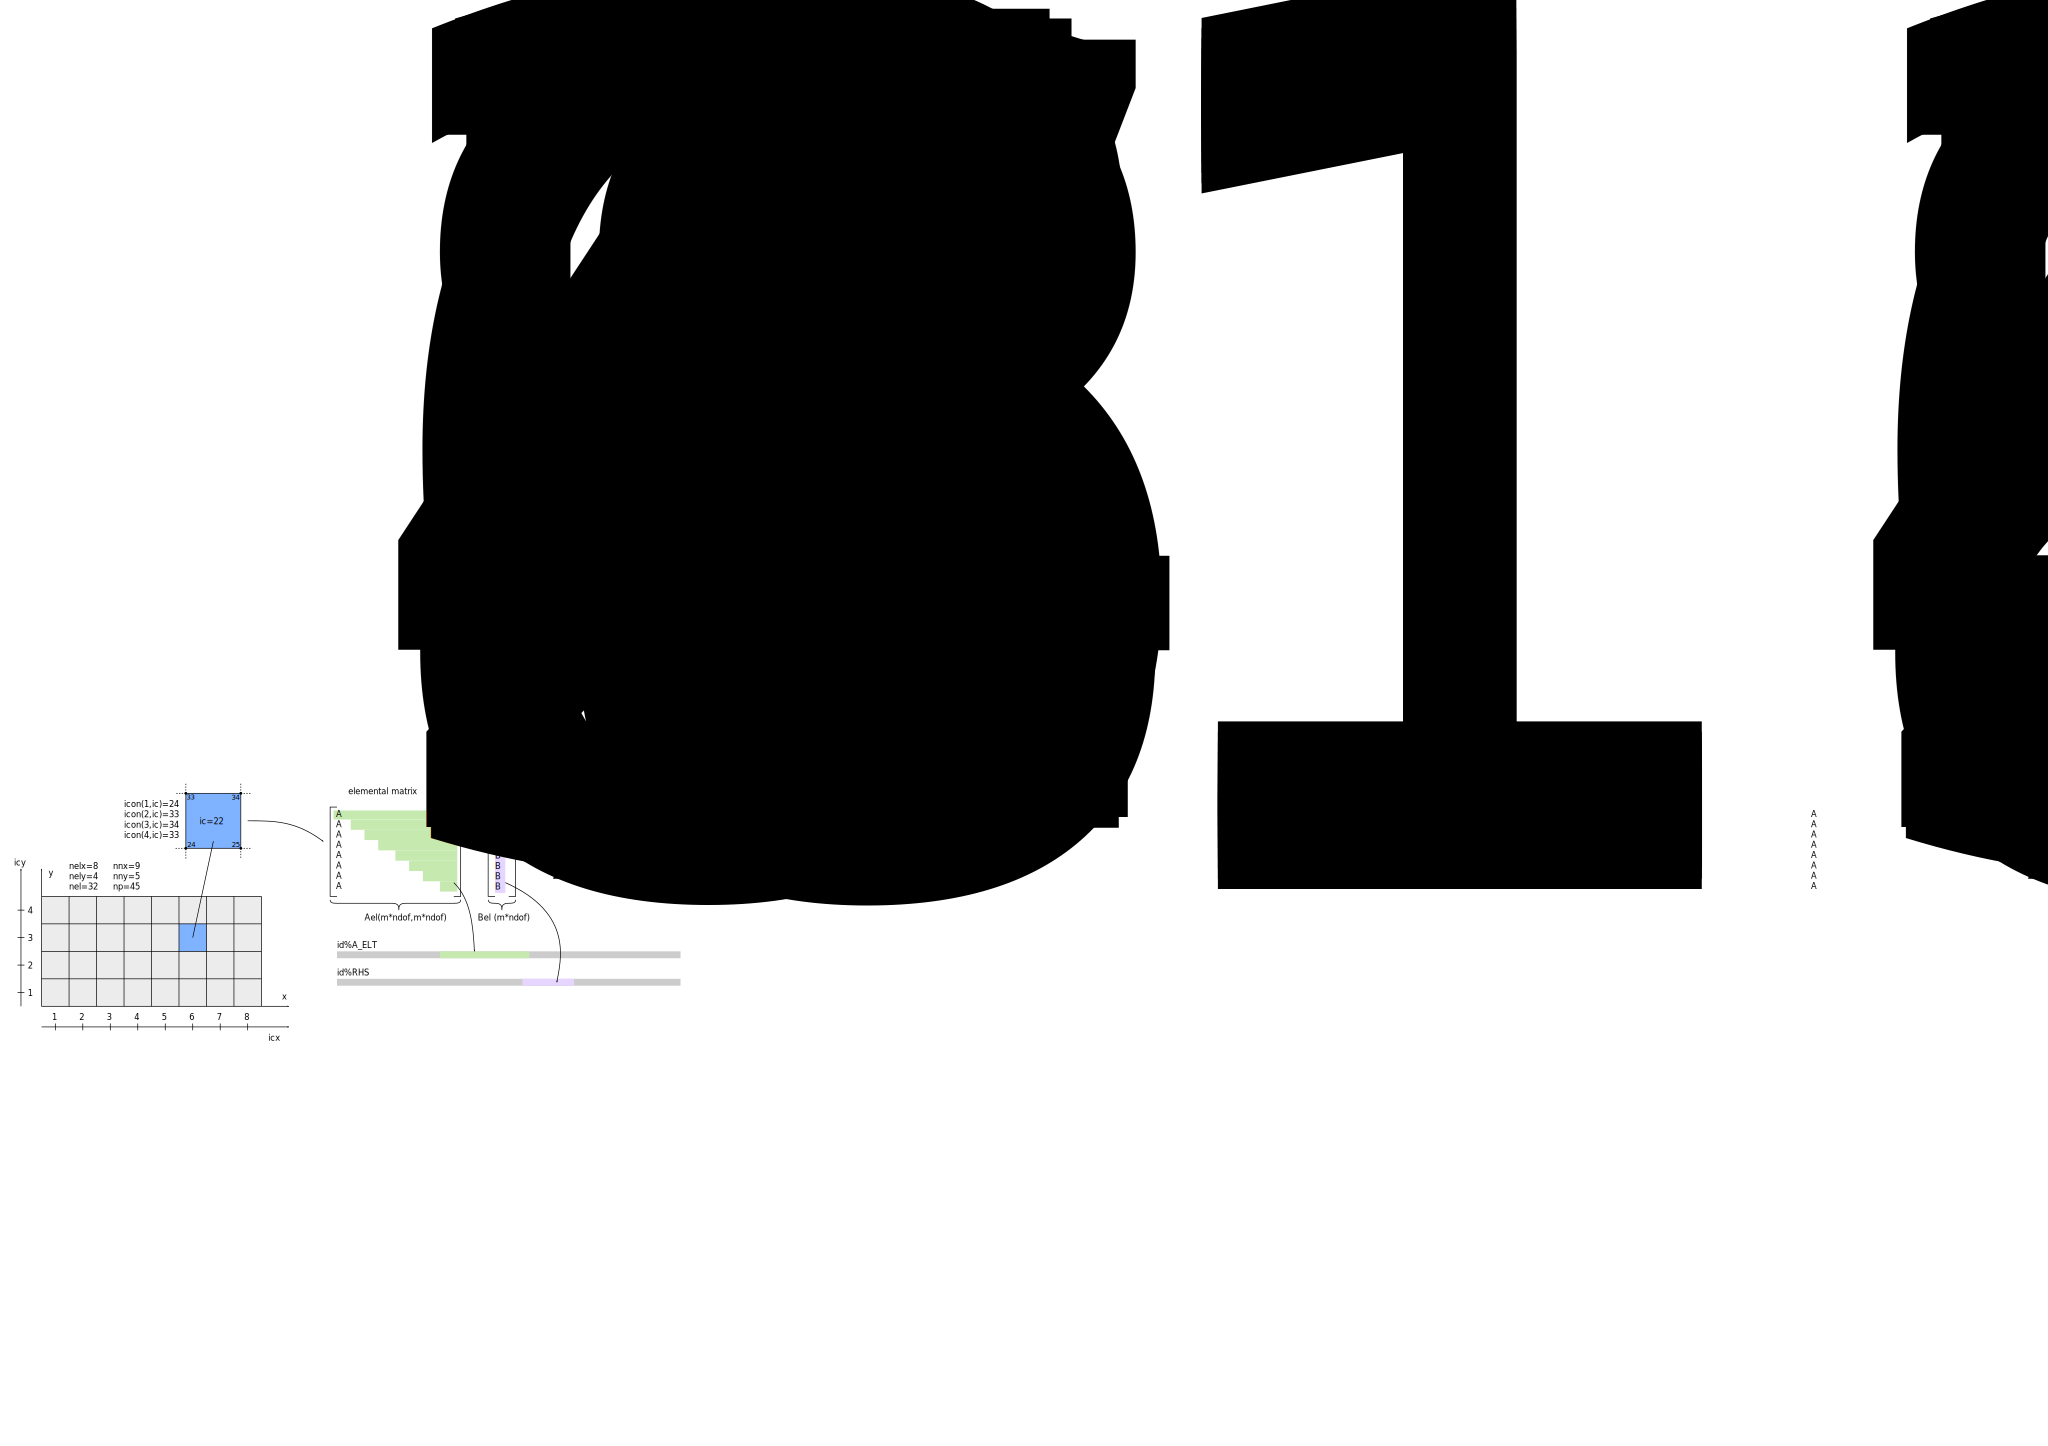
\includegraphics[width=8cm]{python_codes/fieldstone_140/results/exp5/grid}\\
{\captionfont example of regular grid of quadrilaterals split in two triangles}
\end{center}


%................................................................
\section*{Crustal wedge with advection ({\tt experiment=6})}

In this case Lx=200km, Ly=50km. Tectonic advection is included.

\begin{center}
a)\includegraphics[width=8cm]{python_codes/fieldstone_140/results/exp6/uplift}
b)\includegraphics[width=8cm]{python_codes/fieldstone_140/results/exp6/elevation.png}\\
{\captionfont Vertical scale x30. b) after 1000 timesteps = 100,000yr.}
\end{center}

\begin{center}
\includegraphics[width=8cm]{python_codes/fieldstone_140/results/exp6/elevation.pdf}\\
{\captionfont We find the hallmarks of advection: over and undershoots}
\end{center}








%%%%%%%%%%%%%%%%%%%%%%%%%%%%%%%%%%%%%%%%%%%%%%%%%%%%%%%%%%%%%%%%%%%%%%%%%%%%%%%%%%%%%%%%%%%%%%%%%%%%%%%%%%%%%%%%%%%%
\par\noindent\rule{\textwidth}{0.4pt}

\vspace{.5cm}

\begin{center}
\fbox{\begin{minipage}{0.75\textwidth}
To Do \& open questions: 
\begin{itemize}
\item decide/homogenise colorscales for drainage area, slope, elevation...
\item improve speed for gnei and for matrix build
\item test/document Simpson's quadrature?  3 pts see table 7.2???
\item CFL condition ?!
\item benchmarks
\item compute uplift 
\item compute catchment efficiently
\item precipitation fct space coords?
\item cylindrical uplift w, look at average slope
\item avalanche rule, see page 244 of pelletier
\item establish river path ?
\item add nonlinear adv see pelletier ?
\item what physics is in Cascade? \textcite{brsa97}
\item inner lengthscale? one valley increase res?
\item crank-nicolson ?
\end{itemize}
\end{minipage}}
\end{center}

\vspace{.5cm}
\par\noindent\rule{\textwidth}{0.4pt}

\Literature:\\
\fullcite{sisc03}\\
\fullcite{simp04}\\
\fullcite{simp04b}
